\documentclass[11pt,oneside]{book}
\usepackage[a4paper,margin=25mm]{geometry}
\usepackage[T1]{fontenc}
\usepackage[utf8]{inputenc}
\usepackage{lmodern}
\usepackage{microtype}
\usepackage{xcolor}
\usepackage{booktabs,longtable,tabularx,array}
\usepackage{enumitem}
\usepackage{amsmath}
\usepackage{listings}
\usepackage{tikz}
\usetikzlibrary{arrows.meta,positioning,shapes.geometric,fit}
\usepackage{fancyhdr}
\definecolor{hpblue}{HTML}{0B7285}
\definecolor{hpdark}{HTML}{102A43}
\definecolor{hplight}{HTML}{E6FFFA}
\definecolor{codebg}{HTML}{F4F7F9}
\pagestyle{fancy}\setlength{\headheight}{14pt}\fancyhf{}\lhead{HoneyPot System}\rhead{Technical Handbook}\cfoot{\thepage}
\lstset{basicstyle=\ttfamily\small,backgroundcolor=\color{codebg},frame=single,breaklines=true,columns=fullflexible}
\newcommand{\what}[1]{\paragraph{What is it?}#1}
\newcommand{\why}[1]{\paragraph{Why do we need it?}#1}
\newcommand{\how}[1]{\paragraph{How it works here.}#1}
\newcommand{\interview}[1]{\paragraph{Interview explanation.}\emph{#1}}
\newcommand{\statusnote}[1]{\begin{quote}\colorbox{hplight}{\parbox{0.92\linewidth}{\textbf{Implementation status:} #1}}\end{quote}}
\begin{document}
\begin{titlepage}\centering
{\Huge\bfseries HoneyPot System\par}\vspace{7mm}
{\LARGE Complete Technical Handbook\par}\vspace{12mm}
{\large A code-grounded guide to the honeypot, SOC dashboard, detection pipeline, and operations model\par}\vfill
\begin{tabular}{rl}Repository baseline:& \texttt{6cad5b7} (stabilize browser regression suite)\\
Document date:& 29 September 2026\\
Deployment status:& \textbf{Not deployed to the public Internet}\\
Validation status:& \textbf{Mostly validated on native Windows runtime}
\end{tabular}\vfill
\textit{This handbook distinguishes implemented behavior from untested integrations and future work. It does not contain secrets.}
\end{titlepage}
\frontmatter\tableofcontents\listoffigures\listoftables\mainmatter

\chapter{Project Overview}
\what{HoneyPot System is a production-style cybersecurity monitoring platform. Two decoy services collect attacker interaction, FastAPI validates and persists it, deterministic rules create explainable detections and incidents, a Redis-backed worker enriches work, and a Next.js dashboard presents the SOC view.}
\why{A small organization needs visibility into hostile behavior without placing a real production service at risk. A decoy offers controlled evidence of probing, credential guessing, malicious commands, and web attacks.}
\section*{Project in one sentence}An isolated SSH and HTTP deception system turns authenticated attacker telemetry into scored, correlated SOC incidents visible in real time.
\section*{Project in 30 seconds}Attackers interact with fake SSH or HTTP surfaces. The decoys never execute their commands; instead they send normalized events to an authenticated API. Rules detect behaviors such as traversal, SQL injection, brute force, and reverse-shell attempts. PostgreSQL stores evidence, Redis sends background jobs to a worker, and the Next.js SOC dashboard receives live updates through Server-Sent Events (SSE).
\section*{Project in 2 minutes}A Security Operations Center (SOC) is the operational function that watches security telemetry, triages suspicious activity, and tracks incidents. This project implements a compact SOC workflow around safe honeypots. SSH and HTTP decoys capture interaction and post it using a shared sensor key. FastAPI validates the event, creates the attacker/session/event records, evaluates rules synchronously, calculates a transparent score, and correlates related detections from the same IP into a 15-minute unresolved incident. It then publishes a Redis Stream job. The worker optionally enriches the IP, classifies the incident with a persisted logistic-regression baseline, and delivers in-app or configured webhook notifications. Analysts authenticate through a Next.js backend-for-frontend (BFF), investigate events and incidents, acknowledge or resolve them, and see new telemetry by SSE. It is locally validated, but it is \textbf{not publicly deployed}.
\section{Users and use cases}Intended users are SOC analysts and administrators. Analysts investigate events, alerts, attackers, sessions, maps, and incidents. Administrators manage users, rules, and audit logs. The platform is an educational/portfolio system and a controlled sensor, not a replacement for a mature SIEM or an unrestricted malware lab.

\chapter{Cybersecurity and Honeypot Basics}
\what{Cybersecurity monitoring collects telemetry---records about connections, requests, logins, and commands---then turns it into decisions. A SOC is the people, process, and tooling that performs this monitoring. A SIEM-like system centralizes evidence and helps search, correlate, and alert.}
\begin{table}[h]\centering\caption{Core terms}\begin{tabularx}{\linewidth}{lX}\toprule Term & Meaning in this project\\\midrule
Event & One observed action, such as an HTTP request or SSH command.\\
Detection & A rule match attached to an event, with evidence and a score.\\
Alert & An attention signal for a qualifying incident.\\
Incident & Correlated, analyst-managed security case spanning one or more events.\\
Threat & A potential harmful actor or capability; it is broader than a single event.\\
Indicator/IOC & Observable clue such as an IP, path, scanner user-agent, or command token.\\\bottomrule\end{tabularx}\end{table}
\how{A honeypot is a deliberately exposed decoy. It is valuable because interaction should be unusual and therefore useful telemetry. This project captures interaction rather than retaliating, executing code, or claiming attacker attribution. Threat intelligence is optional IP enrichment, not a prerequisite for detection.}

\chapter{High-Level Architecture}
\begin{figure}[h]\centering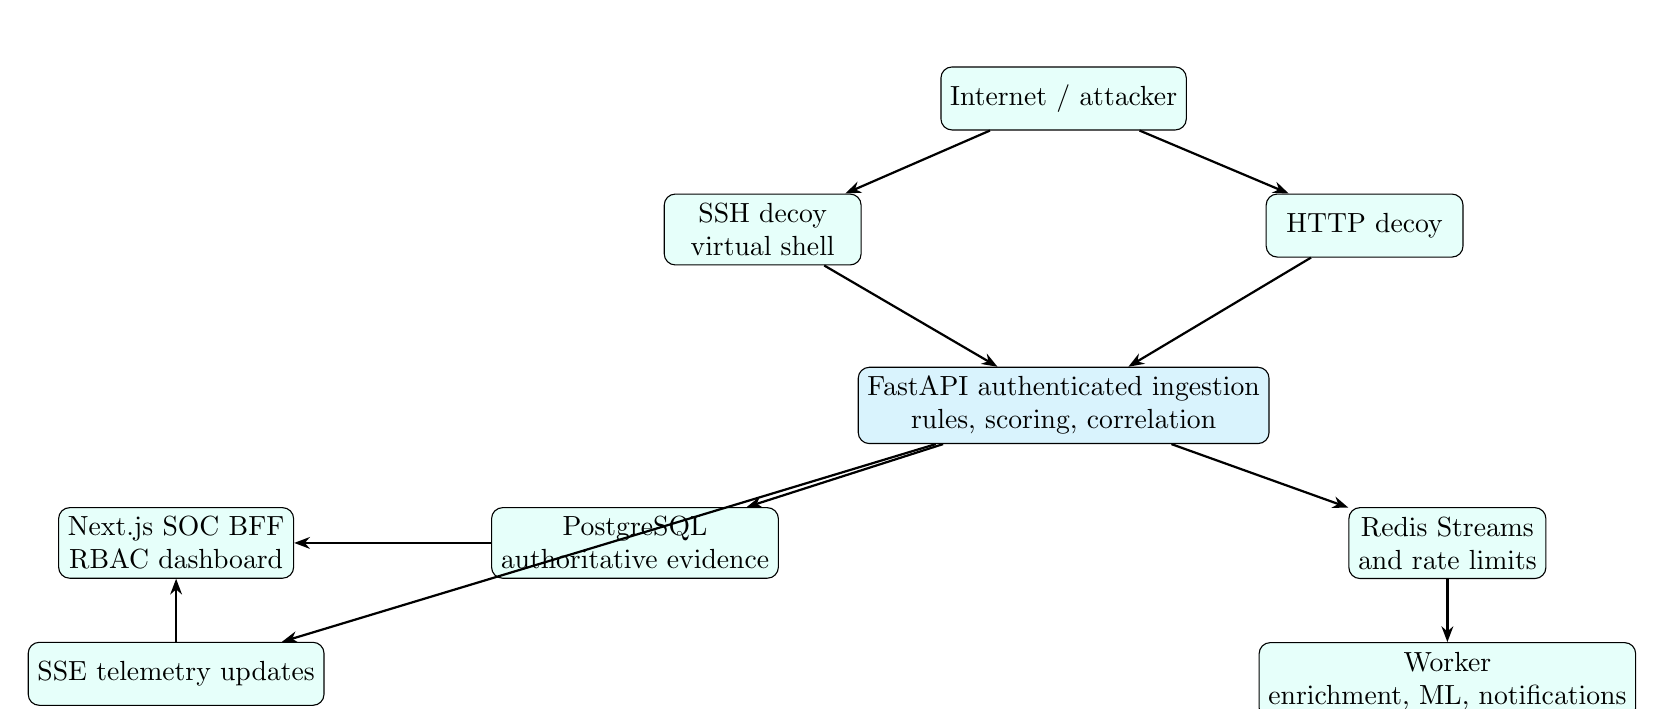
\begin{tikzpicture}[node distance=8mm and 10mm, every node/.style={draw,rounded corners,align=center,minimum width=25mm,minimum height=8mm,fill=hplight}, arr/.style={-{Stealth[length=2mm]},thick}]
\node (attacker) {Internet / attacker}; \node (ssh) [below left=of attacker] {SSH decoy\\virtual shell}; \node (http) [below right=of attacker] {HTTP decoy};
\node (api) [below=of attacker,yshift=-22mm,fill=cyan!15] {FastAPI authenticated ingestion\\rules, scoring, correlation};
\node (db) [below left=of api] {PostgreSQL\\authoritative evidence}; \node (redis) [below right=of api] {Redis Streams\\and rate limits};
\node (worker) [below=of redis] {Worker\\enrichment, ML, notifications}; \node (web) [left=of db,xshift=-15mm] {Next.js SOC BFF\\RBAC dashboard}; \node (sse) [below=of web] {SSE telemetry updates};
\draw[arr] (attacker)--(ssh);\draw[arr](attacker)--(http);\draw[arr](ssh)--(api);\draw[arr](http)--(api);\draw[arr](api)--(db);\draw[arr](api)--(redis);\draw[arr](redis)--(worker);\draw[arr](db)--(web);\draw[arr](api)--(sse);\draw[arr](sse)--(web);
\end{tikzpicture}\caption{Implemented logical architecture. Database and Redis are internal; the dashboard is the analyst UI.}\end{figure}
\how{The API is the trust boundary between sensors and data services. Decoys supply a sensor key but no database or Redis credentials. PostgreSQL stores transactional evidence before background work is queued. Redis decouples slow enrichment from the ingestion response. The Next.js BFF holds browser tokens in HTTP-only cookies and proxies management requests.}
\section{Every arrow}Attacker-to-decoy is untrusted interaction. Decoy-to-API is a normalized, sensor-key-authenticated event. API-to-PostgreSQL is durable event/detection/incident persistence. API-to-Redis is an \texttt{XADD} job plus a publish notification. Redis-to-worker is consumer-group processing. API/database-to-dashboard is authenticated management data through the BFF; API-to-browser is a one-way SSE event stream.

\chapter{Complete Data Flow}
\begin{figure}[h]\centering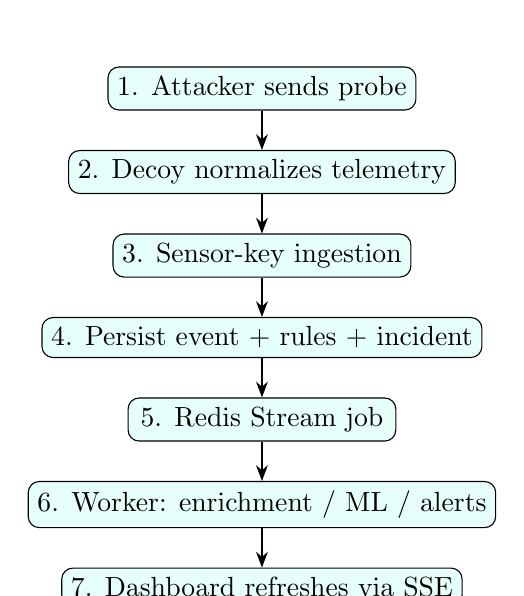
\begin{tikzpicture}[node distance=5mm,every node/.style={draw,rounded corners,align=center,minimum width=34mm,fill=hplight},arr/.style={-{Stealth[length=2mm]}}]
\node (a) {1. Attacker sends probe};\node (b)[below=of a]{2. Decoy normalizes telemetry};\node(c)[below=of b]{3. Sensor-key ingestion};\node(d)[below=of c]{4. Persist event + rules + incident};\node(e)[below=of d]{5. Redis Stream job};\node(f)[below=of e]{6. Worker: enrichment / ML / alerts};\node(g)[below=of f]{7. Dashboard refreshes via SSE};\draw[arr](a)--(b);\draw[arr](b)--(c);\draw[arr](c)--(d);\draw[arr](d)--(e);\draw[arr](e)--(f);\draw[arr](f)--(g);\end{tikzpicture}\caption{Event lifecycle}\end{figure}
\how{The API first rejects oversized bodies and invalid sensor credentials. \texttt{ingest\_event} is idempotent on the supplied event UUID. It upserts the node, attacker, and session; builds 60-second context; evaluates rules; records detections; creates specialized HTTP/command/credential records; correlates an unresolved 15-minute IP incident; and commits. Only after commit does it enqueue background work. If Redis is unavailable, PostgreSQL remains authoritative and the API returns the stored result; worker health exposes the outage.}

\chapter{Frontend: Next.js SOC Dashboard}
\what{The only production frontend is \texttt{apps/web}, a Next.js 16 / React 19 / TypeScript application. It has protected dashboard, events, incident, attacker, session, honeypot, analytics, alerts, threat-intelligence, settings, users, rule, and audit-log routes.}
\why{Next.js provides route structure and server/client rendering boundaries; TypeScript constrains API-shape mistakes; React Query caches and invalidates data. Tailwind supplies consistent utility styling; Recharts renders overview charts.}
\how{The browser calls Next BFF routes under \texttt{/api/management/*}, not FastAPI directly. The BFF forwards the authenticated request. Client views use \texttt{api<T>()}, which applies a 10-second timeout and turns network failure into an \texttt{ApiError(503)}. The overview explicitly renders loading, empty, error, and retry states. There is a global Next error boundary. No production mock-data fallback exists.}
\section{SSE client}The \texttt{LiveListener} opens \texttt{EventSource('/api/management/stream/events')}. On a \texttt{telemetry} event it invalidates overview, events, incidents, and alerts queries. On error it closes the stream, displays reconnecting state, waits one second, and reconnects; the UI also exposes a Reconnect button.
\begin{lstlisting}[caption={Actual SSE client behavior, condensed from \texttt{live-listener.tsx}}]
stream.addEventListener("telemetry", () => client.invalidateQueries({queryKey:["overview"]}));
stream.onerror = () => { stream.close(); setStatus("reconnecting");
  setTimeout(() => setAttempt(value => value + 1), 1000); };
\end{lstlisting}

\chapter{Backend: FastAPI}
\what{\texttt{apps/api} is a FastAPI application with Pydantic request models, SQLAlchemy ORM, Alembic migrations, and routers for health, authentication, ingestion, and management.}
\how{A request flows through CORS and security middleware, a route/dependency, Pydantic validation, business logic, database/Redis access, then a JSON or streaming response. Middleware adds \texttt{nosniff}, \texttt{DENY} framing, and \texttt{no-referrer} headers. Ingestion has content-size and per-minute rate limiting. Management routes require an authenticated user. Health routes expose API, database, Redis, worker heartbeat, and honeypot heartbeat status.}
\interview{FastAPI fits a typed Python service: Pydantic validates boundary data, dependency injection centralizes authentication, and OpenAPI is available during development. It is not selected because it magically secures the system; the routes and dependencies implement the controls.}

\chapter{Authentication}
\what{Authentication answers ``who is this user?'' Authorization answers ``may this user perform this operation?'' The project uses email/password login, Argon2-compatible \texttt{pwdlib} password hashes, JWT access tokens, stored hashed refresh tokens, and one-time reset tokens.}
\how{Login rate-limits an IP/email identity, verifies the hash, writes an audit log, then issues a 15-minute HS256 access JWT containing subject, role, issued-at, expiry, and type. A refresh token is a random value; only its SHA-256 digest is stored. Refresh rotates by revoking the presented record before issuing a new pair. Logout revokes the matching refresh token. The Next BFF uses HTTP-only cookies; \texttt{COOKIE\_SECURE=true} is required for an HTTPS production deployment.}
\begin{figure}[h]\centering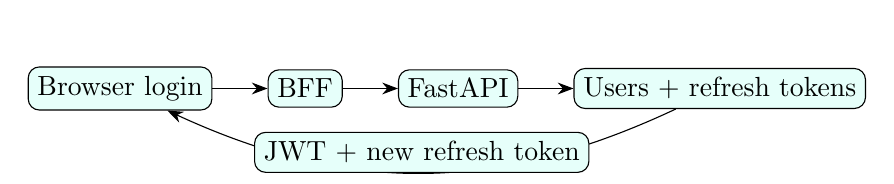
\begin{tikzpicture}[node distance=7mm,every node/.style={draw,rounded corners,align=center,fill=hplight},arr/.style={-{Stealth[length=2mm]}}]\node(a){Browser login};\node(b)[right=of a]{BFF};\node(c)[right=of b]{FastAPI};\node(d)[right=of c]{Users + refresh tokens};\draw[arr](a)--(b);\draw[arr](b)--(c);\draw[arr](c)--(d);\draw[arr,bend left=25](d) to node[above]{JWT + new refresh token}(a);\end{tikzpicture}\caption{Login and token issuance}\end{figure}

\chapter{Role-Based Access Control}
\what{The actual roles are \texttt{ADMIN}, \texttt{ANALYST}, and \texttt{VIEWER}. All management routes require a valid access token.}\how{\texttt{current\_user} decodes the JWT and loads an active user. \texttt{require\_roles} enforces role checks server-side. ADMIN/ANALYST can update incidents and export data; ADMIN creates/updates users and alert rules. A VIEWER may read permitted management data but receives 403 on administration operations. The frontend navigation is a convenience, not the security boundary.}
\interview{Hiding a button is not authorization: a user can call the API manually. The backend must decide.}

\chapter{Password Reset}
\how{A request returns the same generic 202 response whether or not an account exists, reducing account enumeration. For an active user, it generates a random token, stores only its SHA-256 digest with a 30-minute expiry, marks every prior unused reset token as used, and optionally sends the raw token to a private webhook. Confirmation is rate-limited, rejects missing/used/expired tokens, changes the password hash, marks the reset token used, and revokes all active refresh tokens.}
\section{Webhook signing}When configured, the webhook payload is canonical JSON with \texttt{event}, \texttt{delivery\_id}, email, reset token, and issue time. The sender computes \(\mathrm{HMAC\mbox{-}SHA256}(timestamp \mathbin{.} body, secret)\), sends timestamp/signature/delivery-ID headers, and production configuration requires HTTPS and a secret. A receiving webhook must verify signature, freshness, and delivery-ID uniqueness; a receiver is \textbf{not implemented in this repository}, and real delivery was not tested.
\begin{figure}[h]\centering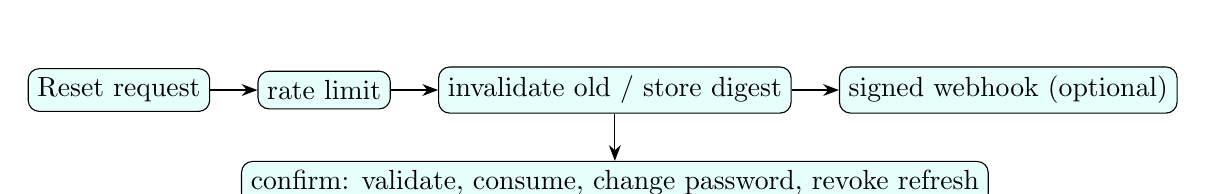
\begin{tikzpicture}[node distance=6mm,every node/.style={draw,rounded corners,align=center,fill=hplight},arr/.style={-{Stealth[length=2mm]}}]\node(a){Reset request};\node(b)[right=of a]{rate limit};\node(c)[right=of b]{invalidate old / store digest};\node(d)[right=of c]{signed webhook (optional)};\node(e)[below=of c]{confirm: validate, consume, change password, revoke refresh};\draw[arr](a)--(b);\draw[arr](b)--(c);\draw[arr](c)--(d);\draw[arr](c)--(e);\end{tikzpicture}\caption{Password-reset flow}\end{figure}

\chapter{Rate Limiting}
\what{Rate limiting caps repeated attempts within a time window, reducing password guessing and reset abuse.}\how{Login (default 10), reset request (5), and reset confirmation (10) use Redis fixed-window keys over the configurable 900-second window. Keys hash \texttt{source\_ip|subject}, so emails are not placed in Redis key names. \texttt{INCR} counts and first use sets expiry. When Redis is unavailable, a process-local deque provides basic protection; it is weaker in multi-instance deployments and health endpoints reveal the outage. Ingestion has a separate per-source per-minute limiter, default 600.}

\chapter{Redis and Redis Streams}
\what{Redis is an in-memory data store used here for short-lived coordination, not the source of security evidence.}\why{PostgreSQL is appropriate for relational, durable incident evidence, whereas Redis is quick for counters, heartbeats, pub/sub, and queued jobs.}\how{After committing an event, FastAPI uses \texttt{XADD honeypot:jobs} with \texttt{kind=enrich\_event}, event ID, and source IP; it also publishes a lightweight notification. The worker creates consumer group \texttt{workers}, reads as a named consumer, acknowledges successful messages with \texttt{XACK}, and sets a 15-second heartbeat. Native validation observed stream entries, one consumer, and zero pending/lag.}

\chapter{Worker}
\what{The worker is a separate Python process for work that should not delay the sensor ingestion response.}\how{For each job, it (1) caches/enriches an IP using an optional configured provider, (2) loads the persisted ML model and writes a prediction for the incident if applicable, and (3) creates in-app notification state and optionally posts an alert webhook. Failures are logged and unacknowledged messages remain available for investigation.}
\interview{Direct API processing is simpler but ties decoy responsiveness to external provider latency and model work. Redis Streams isolate that workload and permit consumer scaling.}

\chapter{PostgreSQL, Migrations, and Data Model}
\what{PostgreSQL is the authoritative transactional record. Alembic migrations \texttt{0001} and \texttt{0002} build the schema; native validation reached revision \texttt{0002}. SQLAlchemy models define fields, foreign keys, relationships, unique constraints, and indexes.}
\begin{figure}[h]\centering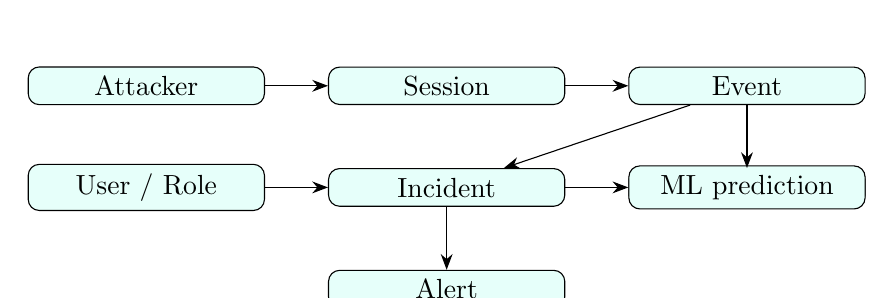
\begin{tikzpicture}[node distance=8mm,every node/.style={draw,rounded corners,align=center,fill=hplight,minimum width=30mm},arr/.style={-{Stealth[length=2mm]}}]\node(a){Attacker};\node(s)[right=of a]{Session};\node(e)[right=of s]{Event};\node(d)[below=of e]{Detection};\node(i)[below=of s]{Incident};\node(al)[below=of i]{Alert};\node(u)[left=of i]{User / Role};\node(m)[right=of i]{ML prediction};\draw[arr](a)--(s);\draw[arr](s)--(e);\draw[arr](e)--(d);\draw[arr](e)--(i);\draw[arr](i)--(al);\draw[arr](u)--(i);\draw[arr](i)--(m);\end{tikzpicture}\caption{Simplified implemented entity relationships}\end{figure}
\begin{longtable}{p{32mm}p{100mm}}\caption{Important persisted entities}\label{tab:entities}\\\toprule Entity & Purpose and key relationships\\\midrule\endfirsthead\toprule Entity & Purpose and key relationships\\\midrule\endhead
roles/users & Unique role name; user email is unique and indexed; a user belongs to a role.\\
refresh\_tokens/password\_reset\_tokens & Token digests, expiry, and revocation/used timestamps; reset and refresh reference a user.\\
honeypot\_nodes/attackers/sessions & Sensor identity, IP identity/enrichment, and a protocol session joining attacker to node.\\
events & UUID event, timestamp, IP, protocol, payload, severity and score. Indexed by timestamp/type and IP/timestamp.\\
command\_events/http\_requests/credential\_captures & One specialized record per relevant event. Credential records preserve a fingerprint; ciphertext is nullable.\\
detections & Rule ID, attack type, score, and evidence for an event.\\
incidents/incident\_events & A numbered IP-based case and its many-to-many event links.\\
alerts/alert\_rules/notifications & Alert lifecycle, configurable threshold rules, and delivery state.\\
threat\_intel/ml\_predictions/audit\_logs & Cached enrichment, persisted prediction inputs/results, and security-relevant user actions.\\\bottomrule\end{longtable}

\chapter{SSH Honeypot}
\what{The AsyncSSH service is a decoy that accepts interaction and exposes a deterministic virtual shell.}\how{It records authentication/commands and sends normalized events through the ingestion API. The shell dispatches an allowlist of simulated commands and response text; it does not call a host shell, subprocess, \texttt{eval}, or \texttt{os.system}. This boundary is essential: an attacker string such as a host escape must be telemetry, never execution. Native validation included a negative host-escape check.}
\statusnote{The decoy is implemented and locally validated. It was not deployed to a public Internet host; public exposure requires separate isolation and host review.}

\chapter{HTTP Honeypot and Ingestion Pipeline}
\what{The HTTP decoy records method, target, query, redacted headers, body size, response code, and session identity. It is useful because scanners and exploit attempts often arrive over HTTP.}\how{Both sensors submit the common event envelope to \texttt{POST /api/v1/ingest/events} with \texttt{X-Sensor-Key}. Pydantic validates fields; body limits and sensor-key comparison protect the boundary. The API creates protocol-specific rows and detects paths, query strings, body previews, commands, and user agents. Sensor heartbeats register/update node name, kind, port, and last-seen time.}
\begin{lstlisting}[language=Python,caption={Actual sensor authentication dependency, condensed}]
expected = get_settings().sensor_api_key.get_secret_value()
if not x_sensor_key or not hmac.compare_digest(x_sensor_key, expected):
    raise HTTPException(status_code=401, detail="Invalid sensor credentials")
\end{lstlisting}

\chapter{Detection Engine}
\what{Rules are deterministic, synchronous, and explainable. They inspect the normalized event plus a 60-second context.}\begin{longtable}{p{35mm}p{51mm}p{15mm}p{35mm}}\caption{All 13 implemented detection rules}\label{tab:rules}\\\toprule Rule & Condition & Score & Action/type\\\midrule\endfirsthead\toprule Rule & Condition & Score & Action/type\\\midrule\endhead
AUTH-BRUTE-001 & At least five auth failures in 60 seconds & 55 & BRUTE\_FORCE\\
SSH-CMD-WGET & \texttt{wget} command token & 35 & suspicious command\\
SSH-CMD-CURL & \texttt{curl} command token & 30 & suspicious command\\
SSH-CMD-CHMOD & executable/777 \texttt{chmod} & 35 & suspicious command\\
SSH-CMD-REVERSE\_SHELL & interactive bash, netcat listener, or \texttt{/dev/tcp} & 60 & suspicious command\\
SSH-CMD-SCRIPT\_EXEC & Python/Perl/Ruby inline execution & 45 & suspicious command\\
CRED-ACCESS-001 & Credential/secret path term & 40 & credential access\\
WEB-SCAN-001 & Sensitive web path; higher after 3 probes & 20/35 & web scanning\\
WEB-SQLI-001 & SQL injection expression & 55 & SQL injection\\
WEB-TRAV-001 & Decoded \texttt{../} or \texttt{..\textbackslash} & 50 & path traversal\\
WEB-CMDI-001 & Shell metacharacter expression & 55 & command injection\\
WEB-UA-001 & Known scanner user agent & 25 & scanner\\
WEB-RATE-001 & At least 30 HTTP requests in 60 seconds & 45 & high-frequency scanning\\\bottomrule\end{longtable}
\statusnote{All 13 rules were exercised through live authenticated ingestion in native validation. Rules are pattern/context detections, not a complete exploit classifier.}

\chapter{Scoring and Incident Correlation}
\how{For matched scores sorted high to low \(s_1,s_2,\ldots\), event risk is \(\min(100, s_1 + \sum_{i>1}\mathrm{round}(0.35s_i))\). Severity is LOW 0--29, MEDIUM 30--59, HIGH 60--79, CRITICAL 80--100. This is visible, auditable logic rather than a hidden model.}\how{A detection event joins the newest unresolved incident with the same source IP and last-seen time inside 15 minutes. A new incident starts at the event score. A later event takes the greater old/new score plus \(\min(10,2\times\text{matched rules})\), capped at 100; attack types become a sorted union. Resolved incidents do not receive correlation.}
\interview{An event is raw evidence; an incident is the analyst's correlated case. For example, traversal and SQL injection from one IP can become one unresolved incident rather than two disconnected tickets.}

\chapter{Alerts and Notifications}
\how{Without configured alert rules, an incident alerts at score at least 80 or for brute force. Configured enabled rules can set a minimum score and optional attack type. The system updates an existing unresolved alert instead of duplicating it. The worker marks an IN\_APP notification delivered and can attempt an optional webhook. Incident acknowledgement/resolution propagates status/timestamps to linked alerts and writes an audit record.}

\chapter{Server-Sent Events}
\what{Real-time communication lets an analyst see new telemetry without a manual reload. Polling repeatedly asks for changes; WebSockets are bidirectional persistent channels; SSE is a simple server-to-browser HTTP stream.}\why{This dashboard primarily needs one-way telemetry notifications. SSE uses browser \texttt{EventSource}, is simpler than a two-way protocol, and works with the existing API stream.}\how{\texttt{GET /api/v1/management/stream/events} reads events newer than a cursor once per second, emits \texttt{event: telemetry} JSON frames, and sends keepalive comments. The client invalidates cached queries and reconnects after errors. Native Playwright validation verified a live count update and SSE reconnect/recovery. The deliberate API-failure dashboard UI browser scenario remains only partially tested.}
\begin{figure}[h]\centering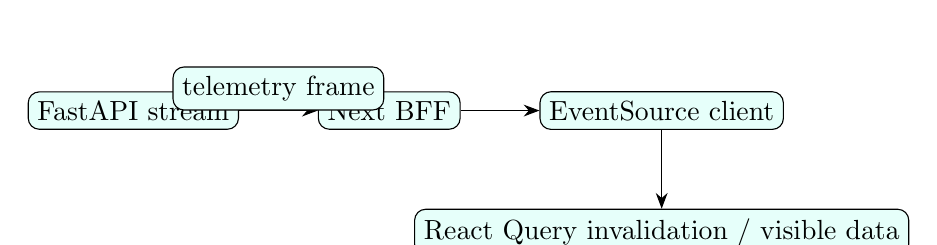
\begin{tikzpicture}[node distance=10mm,every node/.style={draw,rounded corners,align=center,fill=hplight},arr/.style={-{Stealth[length=2mm]}}]\node(a){FastAPI stream};\node(b)[right=of a]{Next BFF};\node(c)[right=of b]{EventSource client};\node(d)[below=of c]{React Query invalidation / visible data};\draw[arr](a)--node[above]{telemetry frame}(b);\draw[arr](b)--(c);\draw[arr](c)--(d);\end{tikzpicture}\caption{SSE update path}\end{figure}

\chapter{Machine-Learning Pipeline}
\what{The ML component is an executable logistic-regression baseline, not the primary detection engine.}\how{The training module generates explicitly synthetic development data, fits a persisted joblib model and writes evaluation JSON. The worker extracts aggregate incident features from linked events, loads the model, calls \texttt{predict\_proba}, and stores classification, confidence, model version, and exact features in \texttt{ml\_predictions}. Logistic regression estimates \(p(y=1|x)=1/(1+e^{-(w^Tx+b)})\); it is interpretable and lightweight.}\statusnote{Model training, persistence, worker load/prediction, and database persistence were validated. The supplied data is intentionally separable synthetic development data. Its metrics do \textbf{not} measure real-world attack detection accuracy.}
\begin{figure}[h]\centering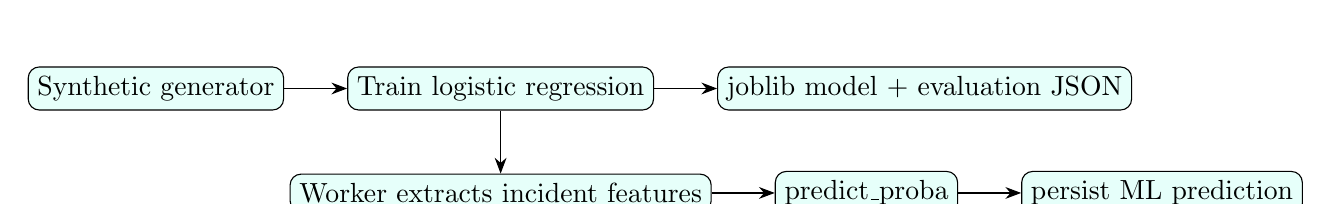
\begin{tikzpicture}[node distance=8mm,every node/.style={draw,rounded corners,align=center,fill=hplight},arr/.style={-{Stealth[length=2mm]}}]\node(a){Synthetic generator};\node(b)[right=of a]{Train logistic regression};\node(c)[right=of b]{joblib model + evaluation JSON};\node(d)[below=of b]{Worker extracts incident features};\node(e)[right=of d]{predict\_proba};\node(f)[right=of e]{persist ML prediction};\draw[arr](a)--(b);\draw[arr](b)--(c);\draw[arr](b)--(d);\draw[arr](d)--(e);\draw[arr](e)--(f);\end{tikzpicture}\caption{Implemented ML lifecycle}\end{figure}

\chapter{Threat Intelligence}
\what{Threat intelligence enriches an observable, here an IP, with external reputation/location data.}\how{The worker uses one generic configured HTTP provider endpoint and bearer key, retries up to three times with short backoff, caches the result for 24 hours, and isolates errors. When available it populates attacker country/city/coordinates/ASN/organization; when unavailable it persists status rather than breaking the job.}\statusnote{The no-provider path was exercised and persisted UNAVAILABLE records. No provider credentials were supplied, so external provider responses were not tested. There are no provider-specific adapters.}

\chapter{Security Architecture}
\begin{figure}[h]\centering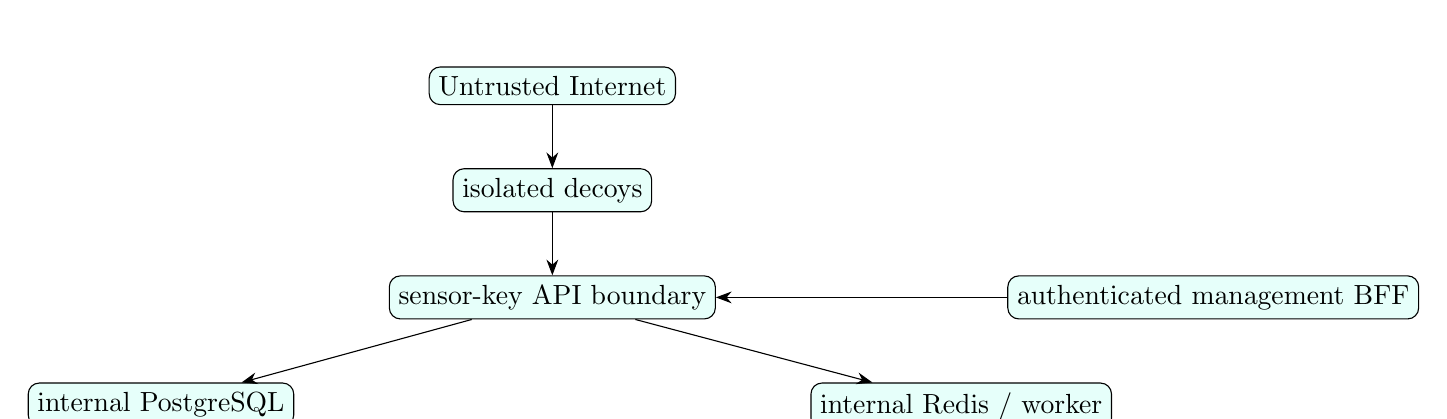
\begin{tikzpicture}[node distance=8mm and 12mm,every node/.style={draw,rounded corners,align=center,fill=hplight},arr/.style={-{Stealth[length=2mm]}}]\node(a){Untrusted Internet};\node(b)[below=of a]{isolated decoys};\node(c)[below=of b]{sensor-key API boundary};\node(d)[below left=of c]{internal PostgreSQL};\node(e)[below right=of c]{internal Redis / worker};\node(f)[right=of c,xshift=25mm]{authenticated management BFF};\draw[arr](a)--(b);\draw[arr](b)--(c);\draw[arr](c)--(d);\draw[arr](c)--(e);\draw[arr](f)--(c);\end{tikzpicture}\caption{Security boundaries: only intended interfaces cross layers}\end{figure}
\begin{longtable}{p{45mm}p{100mm}}\caption{Threat-to-defense mapping}\\\toprule Threat & Implemented defense\\\midrule\endfirsthead\toprule Threat & Implemented defense\\\midrule\endhead
Credential guessing/reset abuse & Redis-backed rate limits; generic reset response; Argon2-compatible password verification.\\
Access-token misuse & Short-lived typed JWT; backend lookup of active user; refresh rotation/revocation.\\
Unauthorized role action & Backend \texttt{require\_roles}, not just hidden UI controls.\\
Webhook forgery & HMAC-SHA256 over timestamp and canonical body; production HTTPS/secret validation. Receiver replay enforcement is external/not implemented.\\
Sensor impersonation & Constant-time sensor-key comparison. Shared key is a documented limitation.\\
Host compromise via decoy input & SSH allowlisted virtual shell; no host command execution; container hardening configuration exists.\\
Oversized/frame/referrer risks & Content limits; nosniff, DENY frame, and no-referrer headers.\\
Data-service exposure & Intended internal network segmentation and loopback native bindings. Public deployment is not performed.\\\bottomrule\end{longtable}
\section{Containers and secrets}Docker configuration uses non-root users, dropped capabilities, no-new-privileges, resource limits, segmented networks, and read-only filesystems where practical. Docker/TLS runtime was \textbf{not tested}. Secrets come from environment variables and must never be committed; production requires unique database password, database/Redis URLs, JWT secret, sensor key, CORS origin, secure cookies, and any webhook secret.

\chapter{Error Handling and Resilience}
\how{The frontend converts fetch failures/timeouts to a recoverable 503-style error and supplies retry UI. SSE provides visible status and reconnection. Ingestion commits PostgreSQL before best-effort Redis enqueue, preserving authoritative event state during a Redis outage; rate limiting has a local fallback. Health endpoints expose database, Redis, worker heartbeat, and honeypot heartbeat. External threat intelligence errors become cached ERROR/UNAVAILABLE state instead of failing ingestion. The worker logs job errors and only acknowledges successful messages.}
\statusnote{Code and focused validation cover these paths. A deliberate browser API-outage UI test remains partially tested; the dashboard should be tested against an actual production failure mode after deployment.}

\chapter{Technology Stack and Rationale}
\begin{longtable}{p{29mm}p{35mm}p{52mm}p{30mm}}\caption{Actual technology stack}\label{tab:stack}\\\toprule Technology & Purpose & Why it fits here & Alternative\\\midrule\endfirsthead\toprule Technology & Purpose & Why it fits here & Alternative\\\midrule\endhead
Next.js 16 / React 19 & SOC UI/BFF & Route structure, React UI, server/client boundaries & Plain React SPA\\
TypeScript & UI correctness & Typed API/UI contracts and refactoring help & JavaScript\\
Tailwind / Recharts & Styling/charts & Fast consistent styling and dashboard visualizations & CSS modules/chart library\\
FastAPI / Pydantic & API/validation & Typed Python routes, validation, dependencies, OpenAPI & Flask\\
SQLAlchemy / Alembic & ORM/schema evolution & Relational mapping and reproducible migrations & Raw SQL/manual schema\\
PostgreSQL & Durable evidence & Transactions, foreign keys, indexes, relational investigations & MongoDB\\
Redis / Streams & Jobs, counters, heartbeats & Low-latency streams and ephemeral coordination & Direct synchronous work\\
AsyncSSH & SSH decoy & Async protocol server with controlled shell integration & Custom SSH protocol\\
scikit-learn / joblib & ML baseline & Mature simple logistic regression/persistence & Heavier ML platform\\
Pytest / Playwright & Testing & Python unit/integration and browser workflow coverage & Other test runners\\
Ruff / ESLint / TypeScript compiler & Static quality & Fast Python and frontend checks & Manual review only\\
Docker Compose / GitHub Actions & Deployment/CI configuration & Repeatable service topology and automation & Manual process management\\\bottomrule\end{longtable}
\interview{PostgreSQL is chosen for durable relationships and incident workflow; Redis complements it for fast ephemeral coordination. Next.js adds a BFF and application routing beyond a plain client-only React app. SSE suits one-way updates; WebSockets would be justified only for richer bidirectional realtime interaction.}

\chapter{Project Directory Structure}
\begin{longtable}{p{43mm}p{100mm}}\caption{Important repository areas}\\\toprule Path & Role and dependencies\\\midrule\endfirsthead\toprule Path & Role and dependencies\\\midrule\endhead
\texttt{apps/api/app} & FastAPI routers, models, schemas, security, detector rules, services; depends on PostgreSQL and Redis.\\
\texttt{apps/api/migrations} & Alembic revision history; deploy with \texttt{alembic upgrade head}.\\
\texttt{apps/worker} & Redis Stream consumer; uses API models and \texttt{ml}.\\
\texttt{apps/ssh-honeypot} & AsyncSSH listener and deterministic virtual shell.\\
\texttt{apps/http-honeypot} & FastAPI HTTP decoy which normalizes requests.\\
\texttt{apps/web/app} & Next routes, including BFF route handlers and protected pages.\\
\texttt{apps/web/components,lib} & Dashboard UI, SSE listener, API client, types/utilities.\\
\texttt{ml} & Synthetic generator, feature extraction, training, evaluation, prediction/model artifact.\\
\texttt{packages/sensor-sdk} & Shared sensor-side event support (used by decoys).\\
\texttt{scripts} & Native Windows setup/start, seed, data generation, and validation scripts.\\
\texttt{docs} & Detection, security, verification, interview, and audit records.\\
\texttt{docker-compose*.yml} & Optional container deployment/hardening topology; not used in native validation.\\\bottomrule\end{longtable}

\chapter{API Documentation}
\begin{longtable}{p{38mm}p{35mm}p{67mm}}\caption{Important implemented API surface}\label{tab:api}\\\toprule Route & Access & Purpose/security notes\\\midrule\endfirsthead\toprule Route & Access & Purpose/security notes\\\midrule\endhead
\texttt{POST /api/v1/auth/register} & Public & Creates user; bootstrap configured first matching email becomes ADMIN.\\
\texttt{POST /api/v1/auth/login} & Public + rate limit & Validates credentials, logs login, returns access/refresh pair.\\
\texttt{POST /api/v1/auth/refresh} & Refresh token & Revokes presented stored token and rotates pair.\\
\texttt{POST /api/v1/auth/logout} & Refresh token & Revokes known refresh record; 204.\\
\texttt{POST /api/v1/auth/password-reset/request} & Public + rate limit & Generic 202; one-time token only for valid active user.\\
\texttt{POST /api/v1/auth/password-reset/confirm} & Public + rate limit & Consumes valid token, changes password, revokes sessions.\\
\texttt{POST /api/v1/ingest/heartbeat} & Sensor key & Upserts decoy node health.\\
\texttt{POST /api/v1/ingest/events} & Sensor key + limits & Validates/idempotently persists event, detections, incident/alert.\\
\texttt{GET /api/v1/management/events} & JWT & Filtered, paginated evidence listing.\\
\texttt{GET/PATCH /management/incidents/:id} & JWT / ADMIN or ANALYST patch & Investigation and lifecycle changes with audit log.\\
\texttt{GET /management/stream/events} & JWT & SSE telemetry stream.\\
\texttt{GET /management/analytics/overview} & JWT & Aggregates for dashboard charts/cards.\\
\texttt{/management/admin/*} & Role dependent & Users/rules/audit logs; mutations require ADMIN.\\
\texttt{/health/*} & Deployment-controlled & API, database, Redis, worker, and honeypot status.\\\bottomrule\end{longtable}
\statusnote{Development OpenAPI is available at \texttt{/docs}; it is disabled when \texttt{ENVIRONMENT=production}. Exact schemas live in \texttt{apps/api/app/schemas}.}

\chapter{Testing and Evidence}
\begin{table}[h]\centering\caption{Recorded validation evidence}\begin{tabularx}{\linewidth}{lX}\toprule Check & Recorded result\\\midrule
Ruff & PASS.\\
Pytest & PASS: 18 tests after auth/reset hardening.\\
Alembic native PostgreSQL & PASS at revision 0002.\\
ESLint / TypeScript / Next production build & PASS.\\
Playwright main workflows & PASS: login, ingestion, investigation, acknowledgement, resolution, major SOC routes.\\
SSE & PASS: live update and reconnect/recovery browser coverage.\\
Native services & PostgreSQL, Redis, API, worker, SSH and HTTP decoys validated.\\
Detection & All 13 deterministic rules validated through live ingestion.\\
ML & Training, persistence, worker prediction, persistence validated.\\
Docker/TLS runtime & Not run; Docker intentionally not installed locally.\\
External intelligence/reset delivery & Not tested without provider/webhook credentials.\\
Controlled API-failure browser UI & Partially tested; no final deterministic browser outage assertion.\\\bottomrule\end{tabularx}\end{table}
\how{Unit tests cover API/auth/detection/decoys/features. Native scripts validate honeypots, detection pipeline, and auth runtime. Playwright covers a browser workflow against the native stack. The report must not be read as an independent penetration test or production deployment validation.}

\chapter{Deployment}
\statusnote{Current status: \textbf{not deployed}. There is no public HTTPS URL and no cloud-provider account/credential configured in the validation environment.}
\how{A future deployment should provision private PostgreSQL and Redis, API, worker, and dashboard services. Run \texttt{alembic upgrade head} against the managed database. Configure unique secrets from \texttt{.env.example}: database/Redis URLs, JWT secret, sensor API key, production CORS origin, secure cookies, optional provider/webhook secrets, and model path. Place an HTTPS reverse proxy or provider TLS endpoint before the management plane. Do not expose PostgreSQL, Redis, worker, secrets, or internal management services publicly. Deploy decoys only on separately reviewed, isolated infrastructure; their host must never execute attacker input.}
\begin{figure}[h]\centering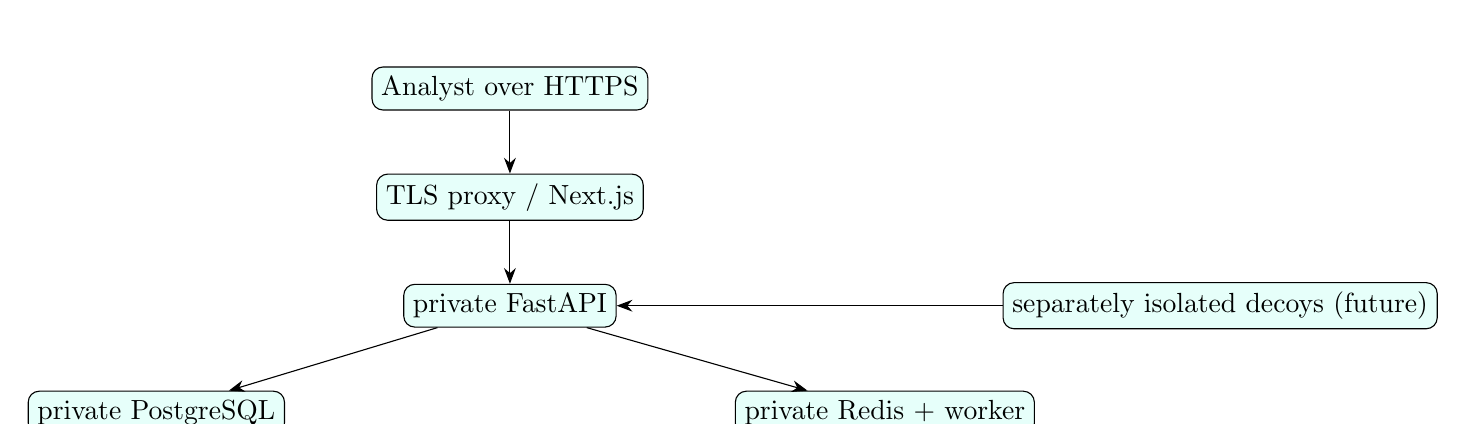
\begin{tikzpicture}[node distance=8mm and 15mm,every node/.style={draw,rounded corners,align=center,fill=hplight},arr/.style={-{Stealth[length=2mm]}}]\node(a){Analyst over HTTPS};\node(b)[below=of a]{TLS proxy / Next.js};\node(c)[below=of b]{private FastAPI};\node(d)[below left=of c]{private PostgreSQL};\node(e)[below right=of c]{private Redis + worker};\node(f)[right=of c,xshift=34mm]{separately isolated decoys (future)};\draw[arr](a)--(b);\draw[arr](b)--(c);\draw[arr](c)--(d);\draw[arr](c)--(e);\draw[arr](f)--(c);\end{tikzpicture}\caption{Target deployment architecture, not a statement of current deployment}\end{figure}

\chapter{Limitations}
\begin{itemize}[leftmargin=*]\item The ML dataset is synthetic; accuracy is not real-world evidence.\item External threat intelligence was not provider-tested.\item Password-reset webhook delivery and receiver-side replay enforcement are not implemented/tested end-to-end.\item The dashboard API-failure UI is only partially browser-tested.\item Docker/TLS container runtime was not tested.\item The platform is not publicly deployed and is not independently penetration tested.\item Sensor authentication is a shared key; per-sensor identities/rotation are future hardening.\item FTP, Telnet, and MySQL decoys are extension points, not implemented services.\end{itemize}

\chapter{Future Improvements}
\statusnote{Everything in this chapter is planned/future work, not implemented functionality.}
\begin{itemize}[leftmargin=*]\item Deploy with private managed data services, HTTPS, backups, monitoring, and a security review.\item Add per-sensor credentials, rotation, mTLS or signed envelopes.\item Build and test a reset-webhook receiver with timestamp age and delivery-ID replay storage.\item Integrate and evaluate real threat-intelligence providers.\item Train/evaluate with governed real-world telemetry and perform drift monitoring.\item Improve correlation across indicators, add queues/metrics/tracing, and integrate with a SIEM.\item Expand safely isolated sensor coverage and distributed worker recovery policy.\end{itemize}

\chapter{Interview Preparation}
\section*{30-second explanation}HoneyPot System is a SOC-style honeypot platform. Safe SSH and HTTP decoys collect attacker actions, FastAPI validates and scores them with deterministic rules, PostgreSQL stores evidence and incidents, Redis sends enrichment jobs to a worker, and a Next.js dashboard gives analysts live SSE updates.
\section*{1-minute explanation}The key design decision is separation: decoys have no database credentials and the SSH shell never executes host commands. Ingestion is authenticated and idempotent. The API synchronously evaluates explainable rules and correlates a source IP's related detections within 15 minutes; the worker handles slower enrichment, ML prediction, and notification. Users get short-lived JWT access plus rotating stored refresh tokens, role checks are enforced at the API, and login/reset operations are rate-limited.
\section*{2-minute explanation}Explain the full flow from decoy interaction to event persistence, rules, score, correlation, Redis job, worker, and SSE dashboard refresh; then call out that rules are primary and ML is a synthetic-data baseline. State clearly that it is locally validated but not publicly deployed.
\section*{5-minute technical explanation}Discuss transactional PostgreSQL persistence before best-effort Redis enqueue, consumer groups/acknowledgement, HMAC reset delivery, backend RBAC, error/retry behavior, and the 13 detection rules. Finish with limitations and deployment isolation requirements.
\begin{longtable}{p{54mm}p{92mm}}\caption{Interview questions and accurate answers}\\\toprule Question & Answer\\\midrule\endfirsthead\toprule Question & Answer\\\midrule\endhead
What exactly does the honeypot do? & It simulates SSH/HTTP services, captures interactions as telemetry, and never executes attacker commands on the host.\\
Why Redis? & Streams decouple background work; counters/expiry support rate limits; heartbeat supports health. PostgreSQL remains authoritative.\\
Why PostgreSQL? & Evidence has strong relationships, transactions, indexes, lifecycle updates, and audit requirements.\\
Why FastAPI? & Typed validation, dependency-based security, async-friendly web framework, and development OpenAPI.\\
Why Next.js? & It structures the dashboard and supplies a BFF so browser management calls need not directly expose backend token handling.\\
How does an event become an incident? & Ingestion validates/persists it, rules produce detections/score, then matching unresolved same-IP detections within 15 minutes correlate into an incident.\\
Why SSE rather than WebSockets? & The implemented requirement is server-to-browser telemetry; SSE/EventSource is simpler for that one-way stream.\\
How is password reset secured? & Generic response, rate limits, random token digest storage, expiry, one-time consumption, old-token invalidation, refresh revocation, optional HMAC-signed delivery.\\
What happens if Redis fails? & Event persistence still succeeds; background enqueue may be skipped, local rate-limit fallback applies, and health reports the outage.\\
What is the ML model/data? & Persisted logistic regression trained on synthetic development data; it validates plumbing, not real-world performance.\\
Is it deployed? & No. The repository was locally validated; no public HTTPS deployment was performed.\\\bottomrule\end{longtable}

\chapter{Glossary}
\begin{longtable}{p{36mm}p{110mm}}\caption{Glossary}\\\toprule Term & Definition\\\midrule\endfirsthead\toprule Term & Definition\\\midrule\endhead
SOC & Security Operations Center: the function that monitors and responds to security telemetry.\\
SIEM & Security Information and Event Management; centralized collection/search/correlation tooling.\\
Honeypot & Controlled decoy intended to observe unwanted interaction.\\
Telemetry & Structured observations emitted by a system or sensor.\\
IOC & Indicator of compromise, an observable clue such as an IP or malicious path.\\
RBAC & Role-Based Access Control: authorization based on assigned role.\\
JWT & Signed JSON Web Token used here for short-lived access.\\
SSE & Server-Sent Events: one-way HTTP streaming from server to browser.\\
Redis Stream & Append-only Redis message stream with consumer-group support.\\
Worker & Separate process that consumes queued work.\\
ORM & Object-Relational Mapping; SQLAlchemy maps Python models to tables.\\
Alembic & Migration tool that evolves the SQL schema reproducibly.\\
CORS & Browser cross-origin policy configured by the API.\\
HMAC & Keyed message authentication code used to authenticate webhook content.\\
Replay attack & Reuse of a previously valid message/token; mitigated by expiry, one-time state, timestamps, and delivery IDs.\\
Rate limiting & Restricting requests per identity/window to slow abuse.\\
Logistic regression & A probabilistic linear classifier used by the synthetic ML baseline.\\
Inference & Applying a trained model to extracted incident features.\\\bottomrule\end{longtable}

\backmatter
\chapter*{Source Basis and Reading Order}\addcontentsline{toc}{chapter}{Source Basis and Reading Order}
This handbook was written from the repository's current source and documentation, especially \texttt{apps/api}, \texttt{apps/worker}, decoy services, \texttt{apps/web}, Alembic migrations, ML modules, \texttt{README.md}, \texttt{docs/DETECTION.md}, \texttt{docs/SECURITY.md}, \texttt{docs/VERIFICATION.md}, scripts, and tests. For a first reading, use Chapters 1--4, 7--13, 17--21, 24, 31, and 35. For code-level preparation, open the referenced source paths alongside the appropriate chapter.
\end{document}
